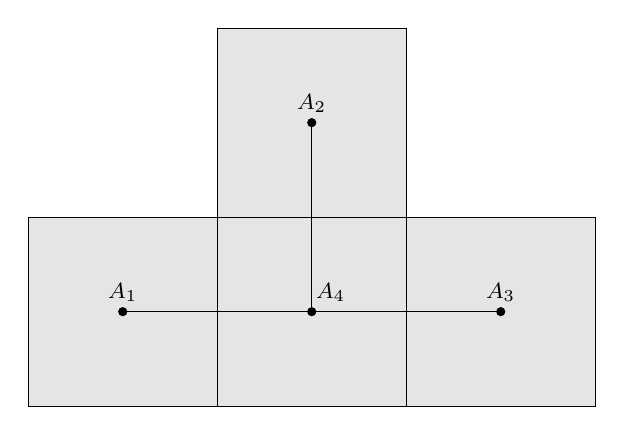
\begin{tikzpicture}[scale=1.2, every node/.style={font=\footnotesize}]
  % Blocchi
  \draw[fill=gray!20] (0,0) rectangle (2,2);  \node at (1,1.2) {$A_1$};
  \draw[fill=gray!20] (2,2) rectangle (4,4);  \node at (3,3.2) {$A_2$};
  \draw[fill=gray!20] (4,0) rectangle (6,2);  \node at (5,1.2) {$A_3$};
  \draw[fill=gray!20] (2,0) rectangle (4,2);  \node at (3.2,1.2) {$A_4$};

  % Nodi del grafo
  \coordinate (A1) at (1,1);
  \coordinate (A2) at (3,3);
  \coordinate (A3) at (5,1);
  \coordinate (A4) at (3,1);

  \draw (A1) -- (A4);
  \draw (A4) -- (A2);
  \draw (A4) -- (A3);

  \foreach \pt in {A1, A2, A3, A4}
    \filldraw[black] (\pt) circle (1.2pt);
\end{tikzpicture}